\chapter{Background - Occupancy-based HVAC Control}
\label{cha:background}

% 1 - Talk the overall picture of occupancy-based HVAC control based on the 5 top things of first figure. Add section to first figure
% 2 - Why the reviewer need to read ur background, why is it important for your thesis... tell them how does the section links to your thesis.. ppl need to understand ur plot. "`This is important because we use it in chapter"' ... 'In chapter 1 we are considering the VAV"', "`In our thesis we adopt this RC thermal model."'
% 3 - Overall too much word, not enough equation... Add equation for R/C 

% --- add alex roger paper in RC

% Todo - 
% 	Link each section to chapters ....
% 	Revise revise revise

% xxxxxxxxxxxxxxxxxxxxxx

% HVAC control - VAV-based system
	% occupancy-based HVAC control
		% conventional control
		% model predictive control
	% adaptive thermal control
	%Link to occupancy-based hvac control, demand control ventilation, basically we focus on demand side building load instead of supply side load.
	% Building thermal dynamics - Wall R/C, occupant heat gain, solar heat gain

% Energy-aware scheduling
	% Meeting scheduling

% xxxxxxxxxxxxxxxxxxxxxx


This chapter provides a comprehensive review on occupancy-based HVAC control, which is the state-of-the-art HVAC control mechanism that optimises energy savings based on occupancy presence in buildings. This control mechanism essentially sets the context and motivation for our problem. Figure \ref{fig:background:config} provides a detailed breakdown of different aspects in occupancy-based HVAC control. These include zone-based HVAC system, occupancy-based control strategy, building thermal network modeling, occupancy modeling and thermal comfort control.

In the following sections, we describe in turn the \emph{zone-based HVAC system} that allows zone-based control, including the HVAC zoning concept, the Variable Air Volume (VAV)-based HVAC system and its operations. Next, we introduce different types of \emph{occupancy-based control strategies}, from traditional strategies, such as On/Off control, proportional–integral–derivative (PID) control, rules-based control that provide coarse-grained control based on static occupancy schedules, to advanced control strategies, such as model predictive  

\begin{figure}[hb]
\centering

\includegraphics[height=2.5in,keepaspectratio]{figs/background_configurations.jpg}	
\caption{Occupancy-based HVAC control}
\label{fig:background:config}
\end{figure}

\noindent control that perform finer-grained control based on the prediction and control of occupancy dynamics in future horizon. We then discuss various \emph{building thermal network modeling techniques} that are used to model building thermal dynamics. These techniques are important to calculate temperature dynamics in each zone and provide as an input to the feedback control system. Following that, we devote a section on \emph{occupancy modeling} and discuss how occupancy dynamics are being gathered, modeled and even proactively controlled to benefit the occupancy HVAC control system. These include using fixed schedule, sensor-based occupancy detection, occupancy prediction and energy-aware occupancy scheduling. Lastly, we talk about \emph{thermal comfort} control using fixed setpoints and adaptive setpoints.


%In Section \ref{cha:bg:hvac}, we describe in turn the HVAC system that allows zone-based control, including the HVAC zoning concept, the Variable Air Volume (VAV)-based HVAC system and its operations. Next in Section \ref{cha:bg:ctrl}, we introduce different types of zone-based control strategies, from traditional strategy that provides coarse-grained control based on static occupancy schedule, to advanced control strategy that performs finer-grained control based on the prediction and control of occupancy dynamics in future horizon. Then we discuss various thermal network modeling techniques that are used to model building thermal dynamics in section \ref{cha:bg:rc}. These techniques are important to calculate temperature dynamics in each zone and provide as an input to the feedback control system. We discuss how occupancy dynamics is being gathered, modeled and even proactively controlled to benefit the occupancy HVAC control system in Section \ref{cha:bg:occ}. Lastly, we talk about thermal comfort setpoint configurations and adaptive temperature control in section \ref{cha:bg:atc}


\section{Zone-based HVAC Systems} \label{cha:bg:hvac}

A zone-based HVAC system provides heating, ventilation and air-conditioning to different parts of a building based on pre-defined building zones. Thermostats are installed at all building zones to measure and feedback zone temperature to the HVAC system. Such zoning systems enable precise control of zone temperature based on occupancy and lead to large savings on energy bills. 

There are essentially two types of zone-based HVAC systems: Constant Air Volume (CAV)-based systems and Variable Air Volume (VAV)-based systems. CAV-based systems provide a constant air flow rate to all building zones but vary the air flow temperature to meet the thermal loads of each zone. VAV-based systems, on the other hand, vary the air flow at a constant temperature (around 13$^{\circ}\mathrm{C}$) and heat up this cold air to a designated temperature based on the heat gains or losses within the thermal zone served. Due to its greater energy savings potential, the VAV-based system is commonly preferred to the CAV-based system in mid-to-large size buildings \citep{sekhar1997critical,yao2007evaluation}.

In our work we focus on VAV-based HVAC systems, which serve over 30\% of the commercial and institutional building floor space in the United States \citep{eia2012cbecs}. These buildings are generally large buildings with a lot of rooms and open spaces with different heating and cooling needs. With VAV-based systems, we demonstrate how energy savings can be achieved by scheduling occupant activities and regulating air flow rate and air flow temperature in advance, in such a way that the VAV-based system is optimised to provide thermal comfort while conserving energy. In the following, we provide an overview of the HVAC zoning system and explain how a VAV-based system operates.% effectively to provide thermal comfort while conserving energy.

\subsection{HVAC Zoning System}

In large buildings, such as commercial offices and university lecture halls, the HVAC system must meet the varying thermal comfort needs of different spaces. The HVAC zoning system is commonly deployed to satisfy these different needs. A building is divided into different areas or ''zones``. A zone can be a single room or cluster of rooms with the same heat gain and heat loss characteristics. The division into zones enables individual control of zones' temperatures. Specifically, the building zones are designed by subdividing each floor into core and perimeter thermal zones. 

\begin{figure}[t]
\centering
\includegraphics[height=3.8in,keepaspectratio]{figs/background_layout.jpg}	
\caption{Typical office floor layout}
\label{fig:background:typical_hvac_zone}
\end{figure}

Figure \ref{fig:background:typical_hvac_zone} shows a layout of office space consisting of multiple perimeter and core thermal zones. %Consider the needs of different zones in a typical office building which have different heat loss and heat gain characteristics. 
The cubicles area and offices are arranged around the outer walls (a.k.a the perimeter zones) of the building, and a number of meeting and utilities rooms are co-located at the inner part of the building (a.k.a the core zone) with no outside exposure. %an inner core of rooms that have no outside exposure. 
% Zoning of HVAC systems typicaly separates perimeter zones that are about 5m deep from those that are in the interior. 

The perimeter zones have at least one wall or window exposed to the outside temperatures. These zones experience different heating or cooling loads based on outdoor conditions. Heat is lost from the heated spaces of the building when the outside air is colder, whilst heat is transferred to the cooler spaces of the building when the outside air is warmer. On top of that, these areas gain or lose heat at a varying rate. For example, the side of a building that is exposed to the sun has more heat gain than the sides that are shaded. The sun position, wall insulation, window build-up and blind shading all effect the heat gain and heat loss of the perimeter zones. Hence, apart from ventilation, these perimeter spaces require either heating or cooling. On the other hand, interior or core zones are unaffected by outdoor conditions and experience more or less constant loads. These zones gain heat from the interior load resulting from the presence of occupants, lights, and equipment. These spaces generally require less heating load but more cooling load. 

The cooling and heating load for both core spaces and perimeter spaces depends on many factors such as occupant density, activity level of occupants (active or passive work tasks), heat produced by equipment, type and level of lighting, and external solar gains. Since different spaces have varying rates of heat gain and heat loss, it is impossible for a HVAC system that delivers a constant volume of air at the same temperature to each corner of a building to provide similar comfort conditions. Therefore, heating and cooling must be supplied at varying rates to different zones of the building. To cater for such complex scenarios, VAV-based HVAC systems capable of providing zone-based control have become a de-facto solution. 


% http://www.achrnews.com/articles/98592-variable-air-volume-systems
%The perimeter zones have at least one wall or window exposed to the outside temperatures. \textcolor[rgb]{1,0,0}{This means that these spaces have more heat loss and heat gain than the interior rooms. On cold days, heat transfers from the heated spaces of the building to the colder outside air (heat loss). On warm days, heat transfers from the warm outside air to the cooler spaces of the building (heat gain). On top of that, these areas gain or lose heat at a varying rate. For example, when the sun strikes one side of a building, that side has more heat gain than the sides that are shaded. The position of the sun, insulation of the wall, amount of window/glass, and blind shading all affect the heat gain/loss of the perimeter zones. These perimeter spaces along the outer walls require either heating or cooling as well as ventilation. On the other hand, the core zones of the building gains heat from the interior load resulting from the presence of people, lights, and equipment. Therefore, these spaces generally require less heating except for a top floor where heat is lost through the roof. The normal condition is that they gain too much heat and therefore require cooling when occupied.} % need to say ventilation?

%The cooling load for both core spaces and perimeter spaces depends on many factors such as occupant density, activity level of occupants (active or passive work tasks), heat produced by equipment, type and level of lighting, and external solar gains. Since different spaces have different rates of heat gain and heat loss, it is impossible for a HVAC system that delivers the same temperature of air at a fixed volume to every space to provide comfort conditions for all of them. Therefore, heating and cooling must be supplied at varying rates to different zones of the building. %A zone is a space or group of spaces in a building with similar requirements for heating and cooling. All rooms in a zone can be supplied with the same temperature supply air at the same flow rate. 
%To cater for such complex scenarios, VAV-based HVAC systems capable of providing zone-based control have become a de-facto solution. 

\subsection{Variable Air Volume (VAV)-based HVAC Systems}

VAV-based HVAC systems \citep{ashrae2016sys} control air from a supply duct and vary the supply air flow and air temperature to each zone based upon the temperature in the building zone. This system is frequently associated to ''zone control`` due to its capability to maintain precise temperature control based on multiple setpoints in individual zones. %A zone can be a single room or cluster of rooms with the same heat gain and heat loss characteristics. 
This system is adopted in our model and the physical model is explained in detailed in Chapter \ref{cha:milp}.
Figure \ref{fig:background:vav} shows a schematic of a VAV-based HVAC system connected to two building zones. 


\begin{figure}[ht]
\centering
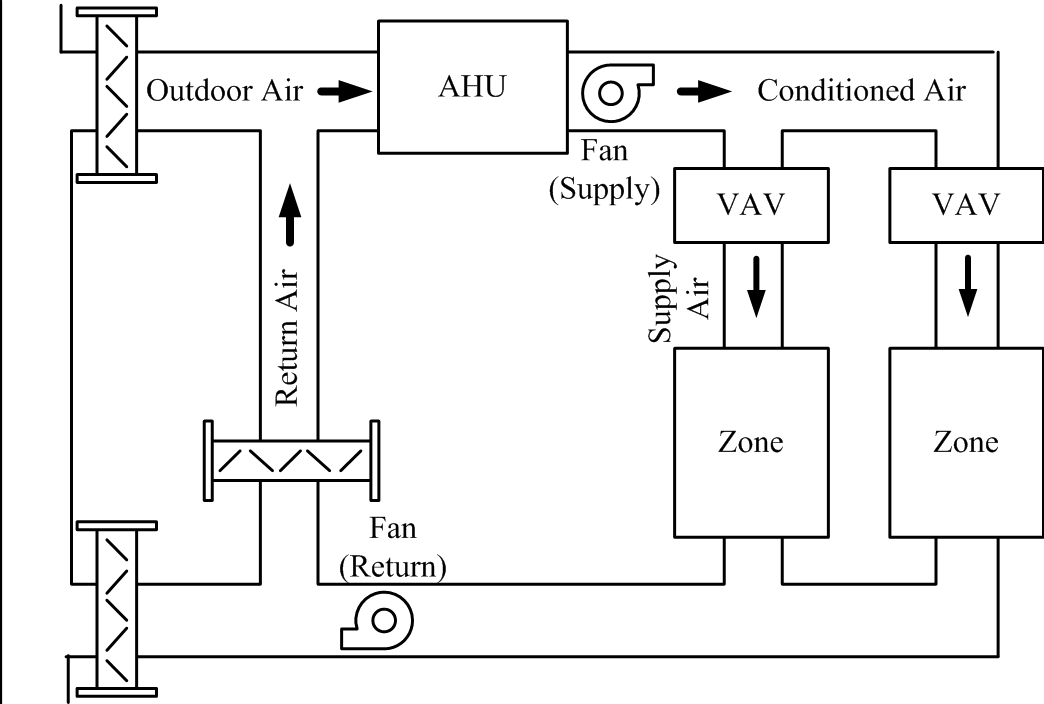
\includegraphics[height=2.3in,keepaspectratio]{figs/background_vav.png}	
\caption{VAV-based HVAC system} 
%  \textcolor[rgb]{1,0,0}{(add controller, air damper, temperature sensor, air flow sensor, actuator)}
% https://necc-controls.com/images/category/vav/johnson-controls-pneumatic_vav.jpg ,  http://www.simplyvav.com/discover/about-vav/
\label{fig:background:vav}  
\end{figure}

The main components are the central air handling unit (AHU), supply fan and VAV units. The AHU admits a mixture of outside air and return air and conditions it to a pre-set conditioned air temperature, usually $12.8^{\circ}\mathrm{C}$. The \emph{\textsl{conditioned air}}\footnote{The \emph{\textsl{conditioned air}} is sometimes referred to ''supply air`` in other literature. However, following \cite{goyal2013occupancy}, we denote as \emph{\textsl{conditioned air}} the cold air distributed by the air handling unit to the supply duct prior to reaching the VAV unit, and as \emph{\textsl{supply air}} the cold air or re-heated air that flows through VAV unit into each zones.} is then distributed through the supply air duct to a network of VAV units in the building. %Each zone has a VAV unit connected to the supply duct. 
A VAV unit is a small metal box located in the supply air duct just before the outlet of each zone. This terminal unit is also called a VAV terminal, VAV box or outlet box. 
The VAV unit is equipped with a few essential components:

\begin {enumerate} [label=\alph*\upshape)] %[label=\itshape\alph*\upshape)]
\item a temperature sensor that monitors each zone temperature,
\item an air flow sensor that monitors the volume of supply air into the zone,
\item an air damper that modulates between open and closed positions to regulate the volume of supply air into the zone,
\item an actuator that adjusts the air damper,
\item the reheat coils that heat up cold conditioned air passing through the air damper into the zone, and 
\item a VAV controller that controls and coordinates all the above operations amongst the VAV components and the AHU.
\end {enumerate} 

\begin{figure}[h]
\centering
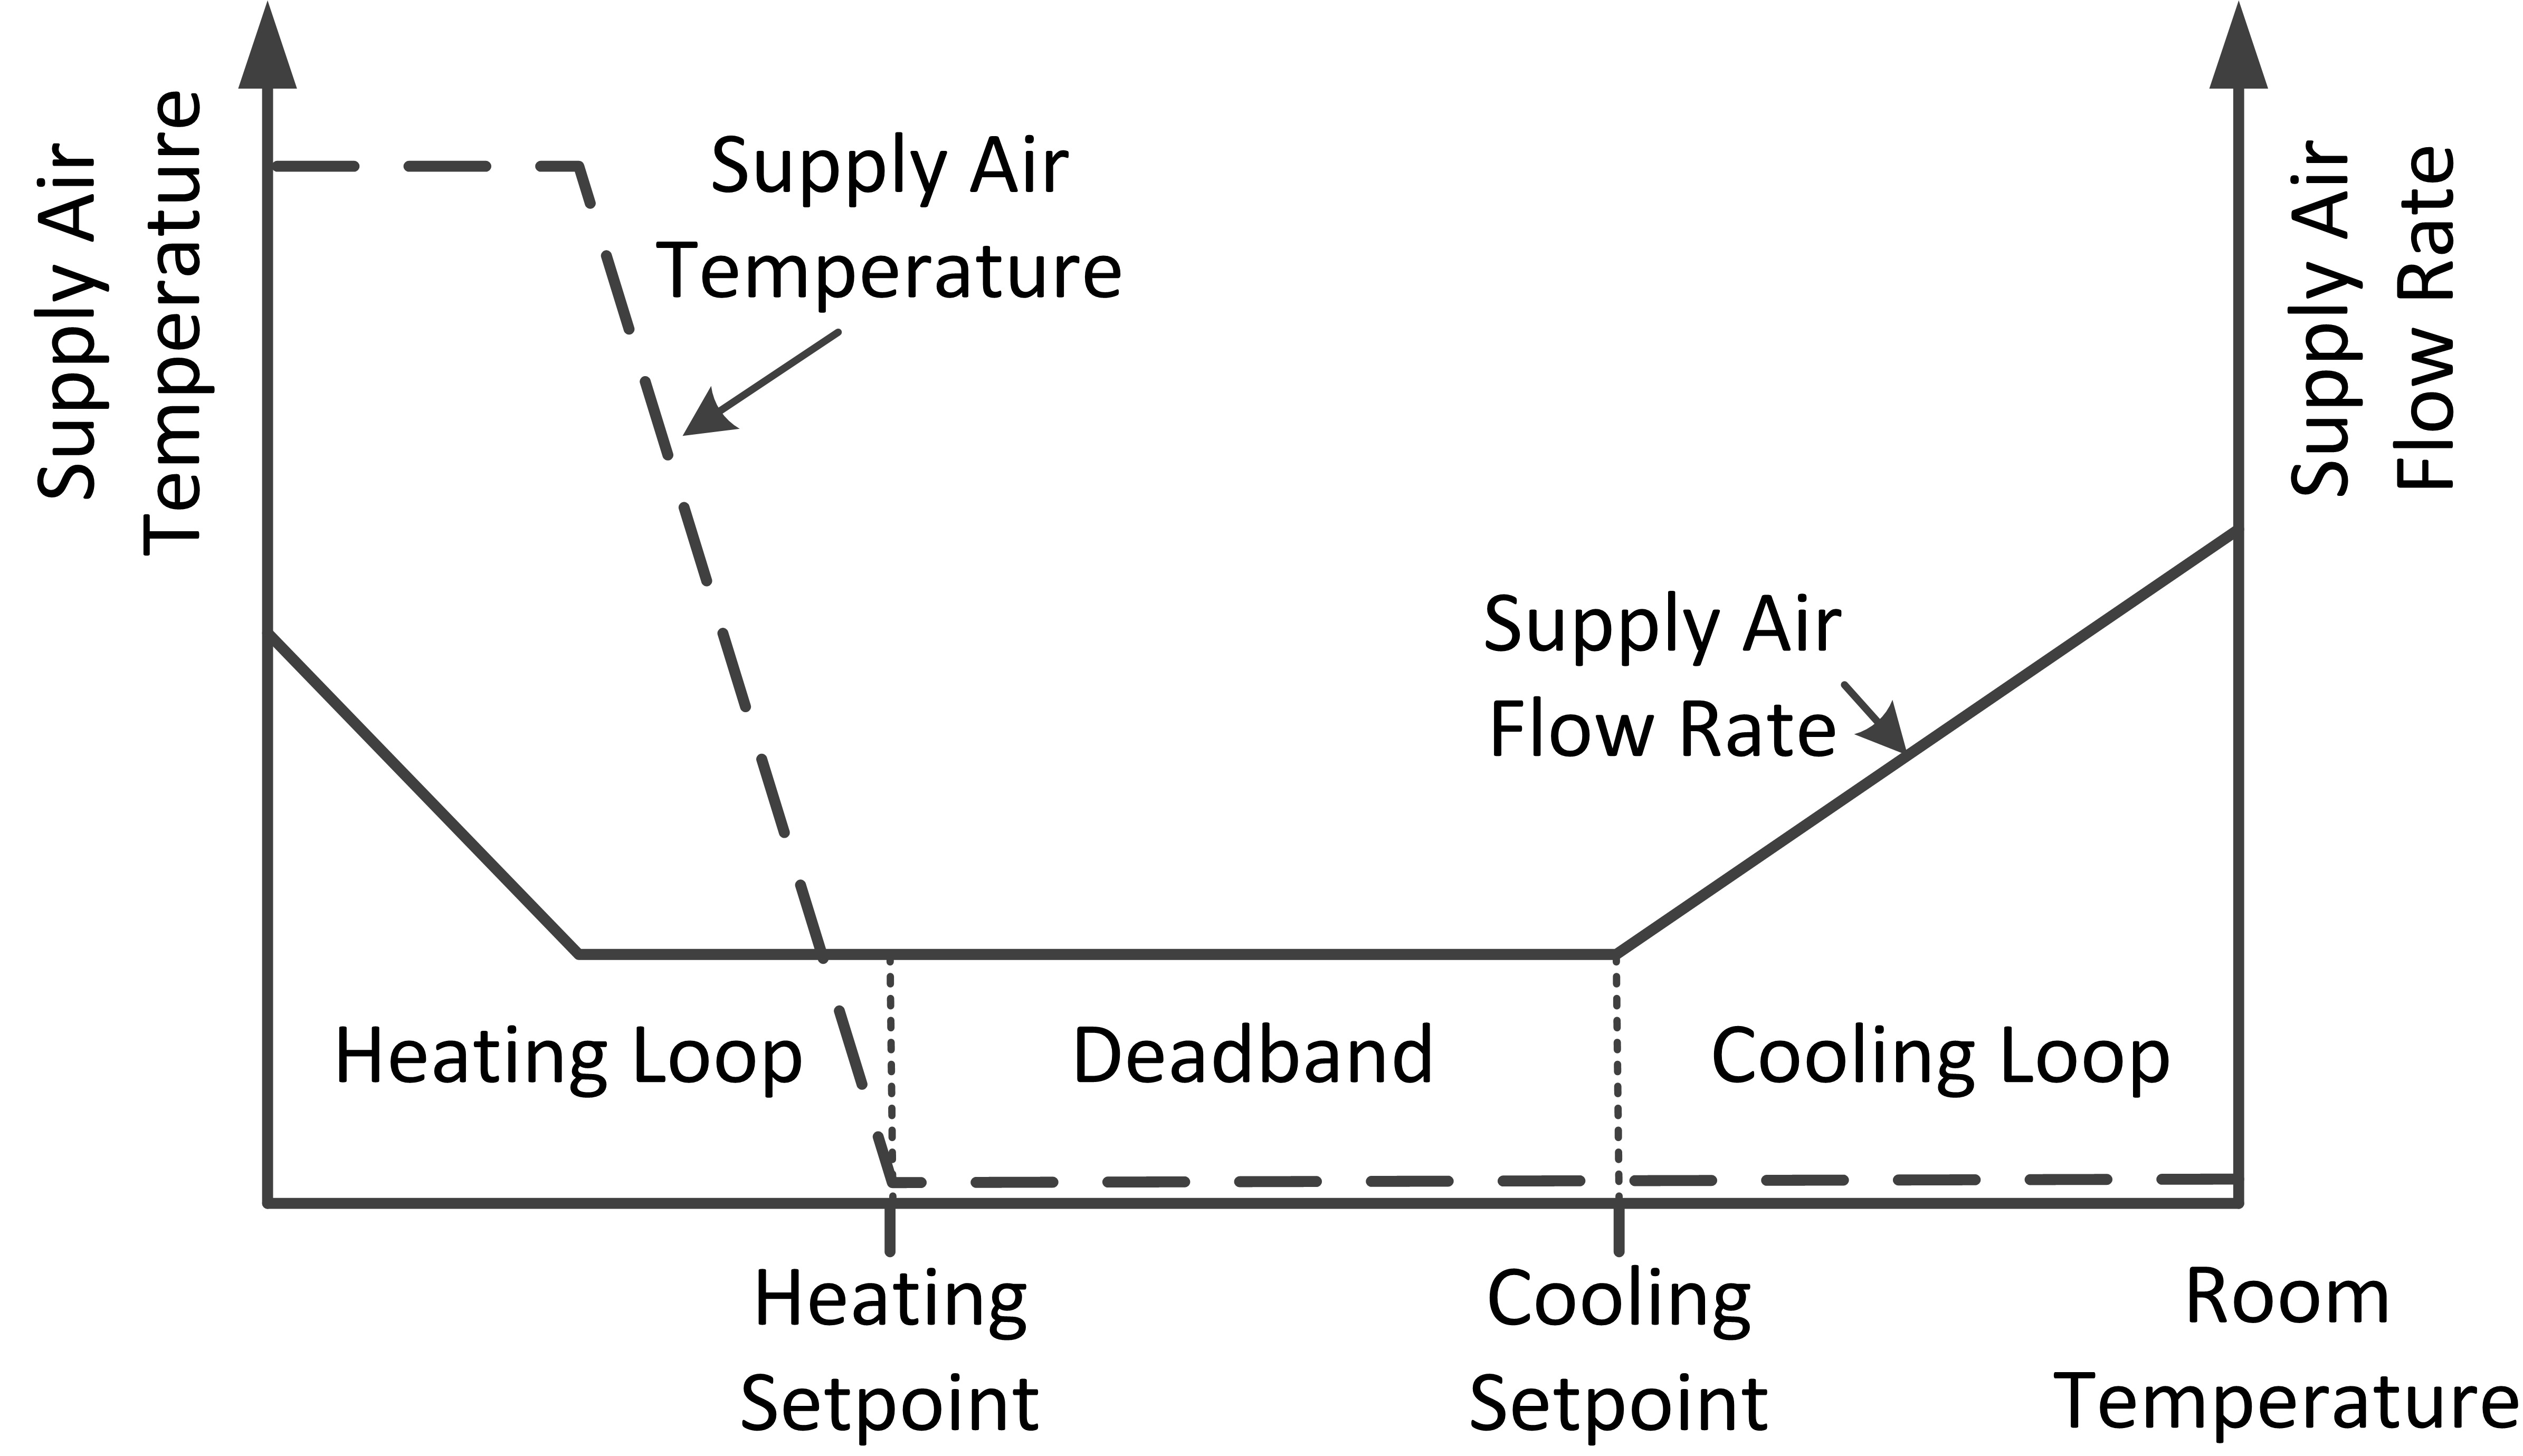
\includegraphics[height=2.5in,keepaspectratio]{figs/background_dualband.jpg}	
\caption{Dual maximum VAV setpoints control logic}
\label{fig:background:dualband}
\end{figure}

Each VAV unit receives conditioned air from the central AHU at the same temperature. As the conditioned air temperature is constant, the \emph{\textsl{supply air}} flow rate and supply air temperature into each zone must vary to meet the rising and falling heat gains or losses within the thermal zone served. Figure \ref{fig:background:dualband} shows a schematic representation of a ''dual maximum`` setpoints control logic used at the VAV units. Each zone has a pre-defined heating setpoint and a pre-defined cooling setpoint. 
In this control sequence, at peak cooling the VAV controller opens the air damper until the supply air flow reaches a pre-defined upper limit. This allows the VAV unit to discharge the maximum amount of cold air\footnote{Ideally the air temperature is similar to the temperature of the conditioned air, or the outdoor air if the temperature outside is cooler than the conditioned air.} into the zone and bring down the zone temperature. As the cooling requirement decreases, the controller modulates the air damper position to decrease the air flow into the zone. When the zone temperature falls between the cooling and heating setpoints, the system enters a deadband mode and is neither heating nor cooling. During this time, the air damper is set to open at a minimum controllable level to allow the minimum amount of air flow into the zone. In the case when a zone temperature falls below the heating setpoint, the system moves into heating mode. The control sequence is broken into two phases. In the initial phase of heating, the air flow will remain at the minimum air flow rate and the reheat coils in the VAV are turned on to add heat to the cold conditioned air up to a designated supply air temperature. If additional heating is required, the air flow rate will increase until it reaches a maximum supply air flow rate. Reheat is typically added to a few perimeter rooms or zones. Although it may seem that heating air that may have been previously cooled is wasteful, using reheat in a few locations may be more economical when both heating and cooling is required from a centralised air supply. %The reheat component is typically an electric resistance element, but hot water coils are also used for reheat.

% When the temperature sensor determines that the zone temperature is within the pre-defined comfort setpoint range, the controller closes the damper in the VAV until the supply air flow reaches a pre-defined lower limit. As the room temperature moves out of the comfort setpoint range, the controller opens the damper until the air flow reaches a pre-defined upper limit, which returns the zone temperature to the setpoint range. The exact position of the air damper varies between minimum air flow and maximum air flow as the requirements for cooling and heating in the room change. In the case when a zone requires heating, the reheat coils in the VAV are turned on to add heat to the cold conditioned air up to a designated supply air temperature. 

%In this control sequence, at peak cooling the air flow setpoint is the maximum amount of air the VAV box is set to deliver. As cooling requirements decrease, air flow decreases until it reaches its minimum setpoint. This setpoint will be based on the minimum controllable level of the VAV box or the required ventilation rate, whichever is higher. When it reaches this minimum, the system is in its deadband and is neither heating or cooling. Up to this point (cooling and deadband) the sequence looks the same as in “single maximum” logic, although the minimum air flow rate is lower. As the system moves into heating mode, the sequence is broken in the two phases. In the initial phase of heating, the air flow will remain at the minimum air flow rate and the reheat valve will modulate to full open. If additional heating is required, the air flow rate will increase until it reaches a maximum heating air flow setpoint. This maximum heating air flow is the same as the minimum air flow rate that is allowed in the “single maximum” strategy. During both of these phases, the VAV box works to maintain a constant supply air discharge temperature to the room. This requires a sensor that monitors the temperature of the supply air discharge. In the heating phases, the supply air discharge temperature should be approximately 90°F; air temperature should not be allowed to get too hot to prevent stratification and short circuiting of the hot air to the return plenum.

As each VAV unit regulates its air flow rate independently, the volume of conditioned air delivered by the central AHU varies according to the demands of the VAV units in the system. This means that the supply fan in the central AHU must vary its output in order to meet the needs of all the VAV units. If the air dampers of most VAV units are fully opened, the conditioned air required for the entire system is high. If most VAV unit dampers are closed, the conditioned air required for the system is much less. Hence the speed of supply fan is regulated to meet the changing demands of the system and to maintain a constant static pressure in the supply duct. 

%The AHU must be able to respond to the fluctuations in duct pressure caused by the individual VAV dampers constantly opening and closing. In addition, it must meet the various demands of individual VAVs. A VAV controller interacts with the AHU through 
%A particular VAV controller does not actually ''force`` the AHU to do anything. Rather it sends requests such as ''send cooler air``. Through its own controller, the AHU determines how to respond to the numerous and varied demands of the VAV units it is serving.

% Instead of just VAV, says  Today, a BAS controls and coordinates VAV, AHU, chiller, boiler etc.
%   https://en.wikipedia.org/wiki/Building_automation
Most VAV systems and the AHU are coordinated and controlled through a centralized building automation system (BAS). Each VAV unit can send information and receive instructions from the BAS, allowing more complex control and optimisation of the HVAC operations. Alternately, the BAS can continually poll each individual VAV controllers, looking for information such as damper position, room temperature, supply air flow rate, and supply air temperature. It can also send remote control instructions to each individual VAV units, such as controlling the damper position, supply air flow rate and supply air temperature into each zone. 

Overall, the main advantage of a VAV-based HVAC system is its capability to ensure occupant comfort and avoid energy waste. Indeed, a building with many VAV zones raises the chances of thermal comfort satisfaction with zone-specific temperature setpoints control. Having many VAV zones also reduces the chance of over-cooling or overheating which lowers fan speeds and lowers the central conditioning requirement, both of which result in lower energy use. 

However, the main issue is that configuring a truly ``high performance'' VAV system, including determining the optimal start/stop of the system, detecting zone occupancy, varying air flow of each zone, optimising fan-pressure optimisation, resetting conditioned-air temperature, optimising zone ventilation etc., is an extremely challenging problem \citep{murphy2011high}. The research and development of these zone-based optimal control strategies has been an ongoing concern in the fields of \emph{\textsl{occupancy-based control}} (OBC) and \emph{\textsl{demand-controlled ventilation}} (DCV), which we describe next %, considering that the zone-based control strategies are essentially depending on the occupancy and the ventilation demands of each zone 
\citep{xu2009model,erickson2010occupancy,liu2012review,balaji2013zonepac,oldewurtel2013importance,goyal2013energy,goyal2013occupancy,zhang2013energy}.

%In the following sections we describe various aspects of occupancy-based HVAC control. We discuss their mechanism, the pros and cons of the system. They range from .... to ....
%Several design and control strategies that can significantly reduce energy use in multiple-zone VAV systems have been proposed. However, implementation of them in buildings seems to be surprisingly infrequent.
%\textcolor[rgb]{1,0,0}{vs .CAV-system, say VAV/CAV are demand side system, there are other supply side system too...}


\section{Occupancy-based Control Strategies} \label{cha:bg:ctrl}

The need for comfort control arises because buildings are occupied.
%The primary reason for building comfort control is because it is occupied.
In practice, however, in the majority of buildings the indoor conditions are either pre-defined or reactive based on temperature sensors. A standard practice is to preset building temperature at a comfortable range, for instance between 20$^\circ$C to 24$^\circ$C during standard operating hours regardless of its occupancy. This practice incurs high energy cost and causes a waste of energy used to heat up or cool down vacant zones. 

The goal of occupancy-based HVAC control is to use occupancy information to reduce energy use -- over conventional control algorithms -- while maintaining thermal comfort and indoor air quality. This control strategy regulates the indoor climate of a building based on either pre-defined, measured or predicted occupancy information. In this section, we discuss various control strategies used to perform occupancy-based control, ranging from conventional control strategies using pre-defined occupancy schedules to advanced control strategies that predict occupancy flow over a control horizon. Conventional controls such as on/off control, PID control and rule-based control are the most commonly used control mechanisms in existing commercial buildings, whilst model predictive control (MPC) is becoming the de facto control strategy in new buildings due to its advanced features that yield higher energy savings.
%Various control mechanisms have been developed to perform occupancy-based control, ranging from basic control strategies that use conventional on/off control, PID control and rule-based control methods, to advanced control strategies that use model predictive control (MPC) approaches. % to optimise HVAC over a control horizon using occupancy information.

Based on the occupancy information, these control mechanisms are used for the dynamic control of the demand-side of the HVAC system, including VAV dampers position control, heating coil control, supply air temperature control, supply air flow rate control and room temperature control. They are also used at the supply side of the HVAC system for controlling the conditioned air temperature set point of an AHU, the chilled water temperature setpoint, the outdoor air ventilation rate and setpoint, the outdoor air damper control, the return air damper control and the supply duct pressure control. As the basic principle of these mechanisms are different, they can accept different level of occupancy details, thereby leading to different granularity of control.

%Conventional controls are the most commonly used control mechanisms in existing commercial buildings. These control mechanisms use classical controllers such as on/off controllers, PID controllers and rule-based controllers to operate HVAC systems. 
\subsection{ON/OFF Control}

The on/off controllers are the most intuitive and easiest to implement. It regulates processes using upper and lower thresholds, and ensures that the control parameters fall within the given bounds \citep{kolokotsa2001advanced,balaji2013zonepac}. Such controllers do not use occupancy measurements. However, they may use pre-defined occupancy schedules. Occupants are usually provided with two types of control flexibilities. They are allowed to change the HVAC occupancy status and the temperature setpoint. For the HVAC occupancy status, there are normally three types of occupancy modes: ``occupied'', ``standby'', ``unoccupied'' \citep{balaji2013zonepac}. By default, the HVAC is always set to ``occupied'' during standard operating hours. During the standard hours in the weekdays, as the zone status is likely to change once it is occupied again, the controller automatically sets itself to ``standby'' mode when the HVAC is off. During the weekends, when the HVAC is turned on, the zone status is changed to ``occupied'' mode for a few hours (for eg. 2 hours or 5 hours). For the rest of the days, the occupancy mode is always set to ``unoccupied''. Although the on/off controller is simple to implement, it fails to react quickly to dynamic processes with time lags, such as HVAC control. The HVAC processes controlled using an on/off controller display large swings from the temperature setpoints.

%The on/off controllers use an upper and lower threshold to regulate the process within the given bounds \citep{kolokotsa2001advanced,balaji2013zonepac}. These types of controllers are the most intuitive and easiest to implement. Such controllers do not use occupancy measurements; though it may use pre-defined occupancy schedules. There are usually two types of control provided to the occupants - changes in temperature setpoint and changes in HVAC occupancy status. For each of the zones, a common temperature setpoint is set. This setpoint is allowed to be changed within a bound from the preset setpoint. There are normally three types of occupancy modes: ``occupied'', ``standby'', ``unoccupied'' \citep{balaji2013zonepac}. The HVAC is always set to ``occupied'' during standard operating hours of the weekdays. When the HVAC is off during the operating hours, the controller automatically sets itself to ``standby'' mode as the zone status is likely to be changed again if occupants come into the zone again. During the weekends, when the HVAC zone is turned on, the zone status is changed to ``occupied'' mode for a few hours (for eg. 2 hours or 5 hours). Although the on/off controller is the most intuitive and easiest to implement, it is unable to control dynamic processes featuring time lags. Because of the high thermal inertia of many HVAC processes, a process that is controlled using an on/off controller displays large swings from the temperature setpoints.

\subsection{PID Control}

The PID controllers modulate controlled variables based on error dynamics to achieve accurate control of a HVAC process \citep{xu2009model,gruber2015energy}. They calculate an error rate based on the difference between a desired setpoint and a measured control variable, and apply a correction to the control variable based on the following proportional, integral, and derivative terms:

\begingroup
\begin{align*}
u_t = K^P e_t + K^I \int_0^t{e_{\tau}} d\tau + K^D \frac{de_t}{dt}.
\end{align*}
\endgroup

\noindent $u_t$ is the control variable at step $t$, $K^P$, $K^I$ and $K^D$ are non-negative coefficients for the proportional (P), integral (I) and derivative (D) terms. $P$ accounts for the present value of the error rate. Based on the model, the control output is directly proportional to the current error rate. $I$ accounts for the past values of the error rate. The integral of the error rate will accumulate over time and impact the control output. $D$ accounts for the future trend of the error rate based on its current rate of change. Using this formulation, the value of the control variable is being adjusted, with an objective to minimise the error rate over time. Note that some systems require only one or two terms to provide appropriate control. This can be achieved by setting the other term(s) to zero. In the absence of the respective terms, a PID controller is called a PI, PD, P or I controller.

PID controllers are effective to develop a supervisory control strategy for HVAC control, such as controlling the position of a damper, or the air temperature setpoint \citep{xu2009model}. For occupancy-based control, the occupancy of each zone and the total occupancy can be given as an input to the control model. This occupancy information can be retrieved from a pre-defined schedule, or measured using occupancy sensors. Generally, the PID controllers return promising results. The drawback of this model is that $K^P$, $K^I$ and $K^D$ require tunings. Thus, they are not resilient to disturbance and the performance of the controllers degrade when the operating conditions vary from the tuning conditions.
%\textcolor[rgb]{1,0,0}{The PID controllers use error dynamics and modulate the controlled variables to achieve accurate control of the process \citep{xu2009model,gruber2015energy}. These mechanisms are effective to develop a supervisory control strategy for HVAC control, such as optimising the conditioned air temperature set point of an AHU, the chilled water temperature setpoint and the outdoor air ventilation rate \citep{xu2009model}. Occupancy information can be pre-defined in a schedule, or measured using occupancy sensors. The occupancy of each zone and the total occupancy are given as an input to the control model. These controllers produce promising results, but tuning the controller parameters, such as the parameters of the cooling coil and fans, the building cooling load, pollutant load etc, is cumbersome. They are also not resilient to disturbance and the performance of the controllers degrade if the operating conditions vary from the tuning conditions. }

\subsection{Rule-based Control}

The rule-based controllers determine all control inputs based on a series of rules of the form ``if \textsl{condition}, then \textsl{action}'' \citep{dhummi2011robust,agarwal2011duty,goyal2012zone,goyal2013occupancy}. The rule-based controller in \cite{agarwal2011duty} uses occupancy measurements to turn off the HVAC system, while the controller in \cite{dhummi2011robust} modulates the supply air flow rate and the zone temperature setpoints in each zone based on measured occupancy. \cite{goyal2013occupancy} defines a set of rules to control zone temperature setpoints during occupied and unoccupied periods. Their controller is designed such that the temperature setpoints are allowed to fluctuate within a larger range when the measured occupancy is zero, and are tightened when the measured occupancy is more than one. Furthermore the controller calculates the minimum supply air flow rate based on the number of occupants in the zone. The decision of temperature setpoints is crucial as a wider range will reduce energy consumption in general, since the controller may be able to reduce reheating during low thermal load conditions and reduce the air flow during high thermal load conditions. Too wide a range, however, will lead to discomfort of the occupants. Therefore, for these types of controllers, the conditions and actions are usually associated with numerical parameters (e.g. threshold values) that need to be chosen. A good performance of the rule-based controllers critically depends on a good choice of rules and associated parameters. 

\subsection{Model Predictive Control}

Unlike conventional control mechanisms, MPC is an advanced method which uses a system model to predict the future states of the system and generates a control vector that minimises a certain cost function over the prediction horizon in the presence of disturbance and constraints. 
The optimisation model can be formulated in general form as follows:

\begingroup
\begin{align*}
\min \quad &f\left(x_{t\rightarrow t+N|t}, u_{t\rightarrow t+N|t}\right) \\
\mbox{subject to} \quad &x_{t+k+1|t} = g\left(x_{t+k|t}, u_{t+k|t}\right) \quad k=\left[0, 1,\ldots, N-1\right] \\
&x_{t+k|t} \in X \\
&u_{t+k|t} \in U \\
%\mbox{min} \quad &c^Tz	\\
%\mbox{subject to} \quad &Az = u	\quad \mbox{(linear constraints)} \\
%&\undersl{z} \leq z \leq \oversl{z}	\quad \mbox{(bound constraints)}\\
%\mbox{\emph{some or all }} &z_i \mbox{\emph{ must take integer values} \quad (integrality constraints)}
\end{align*}
\endgroup

\noindent where $x_{t+k|t}$ denotes $(t+k)$th predicted state of the system at step $t$. $u_{t+k|t}$ represents the exogenous input to the system, calculated at step $t$. The HVAC system's state trajectories are explored based on initial states and predicted disturbances (i.e. inputs) to the system, and a cost-minimising control strategy is identified until time $t+N$. 
%Only the results at step $t$ is introduced to the system as optimal inputs. 
Only the decision for time step $t$ is executed.
The prediction horizon is then shifted forward and the process is repeated all over again to calculate the optimal control signal.

Using MPC, constraints can be placed on the rate and range limits of the controlled variables (e.g. the upper and lower limits of the zone temperature, supply air flow rate limits, and range and speed limits for damper positioning). External and internal disturbances such as weather, occupant activities and equipment can also be modeled, and their predicted effects on the system are used during control vector computation. This effort results in a controller that regulates the process tightly within the given bounds, and is robust to both time-varying disturbances and system parameters. 

The main advantage of MPC is the fact that it allows the current time step to be optimised, while taking future time steps into account. This is achieved by optimising a finite time-horizon, but only implementing the control variables of the current time step. In contrast to the conventional controllers that do not have this predictive ability, MPC has the ability to anticipate future events and can take control actions accordingly. 

When applied to occupancy-based HVAC control, MPC employs a discretized model of the HVAC system, the building thermal dynamics, and exogenous inputs such as outdoor weather, solar gain, zone heat load (occupancy and equipment). It solves an optimisation problem to determine the optimal HVAC control while meeting the occupants' comfort requirement \citep{sun2010integrated,oldewurtel2010energy,nghiem2011receding,ma2011distributed,mady2011stochastic,oldewurtel2012use,goyal2012effect,oldewurtel2013importance,goyal2013occupancy,parisio2013randomized,zhang2013scenario,west2014trial,brooks2015energy}. 

Specifically, in the MPC model, the occupancy information is provided as an exogenous input. This information can be obtained from a pre-defined schedule, or predicted based on occupancy models generated using methods in Section \ref{cha:bg:occ}. The number of occupants are used to project occupancy heat gain based on the occupant activity level. For example, \cite{ashrae2013thermal} states that each occupant generates about 60W-120W based on their activity level in the office. Based on this occupancy information, the MPC model optimises the HVAC control by pre-cooling or pre-heating the room temperature to a certain comfort level prior to the projected occupied hours, while otherwise the room would stay at its setback temperature.

Conventional control methods such as PID control and rule-based control are easy to implement since they are pure feedback strategies based on measured temperature and occupancy. MPC, in contrast, requires additional information of the HVAC model, the building dynamics and the predictions of exogenous inputs such as occupancy information. Despite its computational complexity and the need for a good building thermal dynamic model, however, the MPC models reduce energy use significantly compared to conventional control schemes that are currently used to operate buildings \citep{oldewurtel2010energy,mady2011stochastic,goyal2013energy,goyal2013occupancy,brooks2015energy}. These models consistently incorporate occupancy information into the control and yield an optimal control of the building for a given occupancy prediction over sufficiently long prediction horizon; independently of any parameters and threshold values that are required to be tuned for PID control or rule-based control. In spite of high degree of uncertainty in building dynamics and exogenous inputs, \cite{goyal2012effect} and \cite{zhang2013scenario} show that MPC controller performance is robust to uncertainties, making it a good candidate for building control. 
We refer readers to \citep{afram2014theory,mirakhorli2016occupancy} for comprehensive reviews of MPC-based HVAC control methods.

% Refer to \citep{cigler2013beyond} talk more details about challenge in MPC.
MPC is adopted in our model and the details are explained in Chapter \ref{cha:milp} Section \ref{sec:mip:control}. 
The challenge of MPC is that it requires an appropriate model that adequately captures the thermal dynamics of the building, which is then used for the computation of the optimal control inputs to the zone temperatures \citep{cigler2013beyond}. This model must be sufficiently precise, in order to yield valid predictions of the relevant variables (e.g. room temperatures), but at the same time, the model must be as simple as possible for the optimisation task to be computationally tractable. %and numerically stable. 
%In Section \ref{sec:mip:control}, we show how model predictive control is adopted in our joint occupancy scheduling and HVAC control model, and how the challenge is being tackled. 
In the next section, we discuss various building thermal models, specifically the lumped RC model that is used to simulate the transient thermal dynamics of a building in our work.

%\textcolor[rgb]{1,0,0}{Say we use MPC and thermal model is an important component for MPC}In the next section, we discuss various building thermal models, specifically those that are used to simulate the transient thermal dynamics of a building in our work. % that relates the control signals to the space temperature.


\section{Building Thermal Network Modeling} \label{cha:bg:rc}

The dynamics of temperature evolution in a building is one of the most complex aspects of the overall building dynamics. The complexity lies in modeling the thermal interactions amongst rooms, occupants, equipments, outdoor climate conditions and HVAC system. The thermal interactions in a multi-zone building can be thought of as an interconnected system of many subsystems. Each subsystem corresponds to a zone, and the interconnections correspond to dynamic interactions between pairs of zones. These interactions can be either 
\begin{itemize}
	\item through conduction through the walls, 
	\item through convective air exchange among rooms or,
	\item through radiation from various material interfaces (e.g. walls, equipments and occupants). 
\end{itemize}
\noindent Incorporating these interactions in a building thermal model is a challenging task since it requires modeling heat exchange through convection, conduction and radiation among all adjacent rooms. A first-principles based model constructed from energy and mass balance equations that model all these behaviors will lead to a highly complex model \citep{goyal2012method}. 

Alternately, simpler building thermal models are sought of to simulate the thermal dynamics without losing its practicability \citep{kramer2012simplified,cigler2013beyond}. A lot of efforts have been devoted to modeling simplified building thermal network model that are applicable to computationally intensive HVAC control model, such as MPC. 
%Much effort has been devoted to modeling simplified building thermal response that are applicable for computational intensive model-based HVAC control, such as MPC. 
These simplified models include response factor methods \citep{mitalas1967room}, conduction transfer functions \citep{stephenson1971calculation}, finite difference methods \citep{clarke1985energy} and lumped resistance-capacitance (RC) methods \citep{crabb1987simplified}.

\subsection{RC Model}

%\textcolor[rgb]{1,0,0}{First explain equation of R and C, refer Gouda
%Second, put black box before grey box. Say we use white box, and say we adopt black box in EP chapter}

In our work, we focus on the lumped resistance-capacitance (RC) method.
%An extensive literature exists on modeling the conductive interaction between two spaces though the wall separating them. The most popular modeling framework consists of using resistors and capacitors to model this interaction \citep{}. 
The model is built analogously to the electrical network analogy: a thermal resistance is represented by \textsl{R} (analogously to electrical resistance) and a thermal capacitance is represented by \textsl{C} (analogously to electrical capacitance). The connecting edges represent heat flow, characterised by a temperature.
This method models building thermal response by breaking up construction elements into a number of temperature-uniform elements, about which the transient heat flow through a solid surface, such as a wall or a window, can be expressed. 
Figure \ref{fig:background:walls} depicts a construction element consisting of multiple layers of different building materials. Depending on the materials used, each layer has different thickness, thermal conductivity, specific heat capacity and density. With the lumped RC method, such construction element consisting of \textsl{n} layers of materials can be combined to form $n$ ``lumped'' thermal resistances (R) and $n-1$ ``lumped'' thermal capacitance (C). Figure \ref{fig:background:rc} illustrates an example with three ``lumped'' thermal resistances ($R^z_l$, $R^{mid,z}_l$, $R^l_z$) and two ``lumped'' thermal capacitance ($C^z_l$, $C^l_z$).

\begin{figure}[h]
\centering
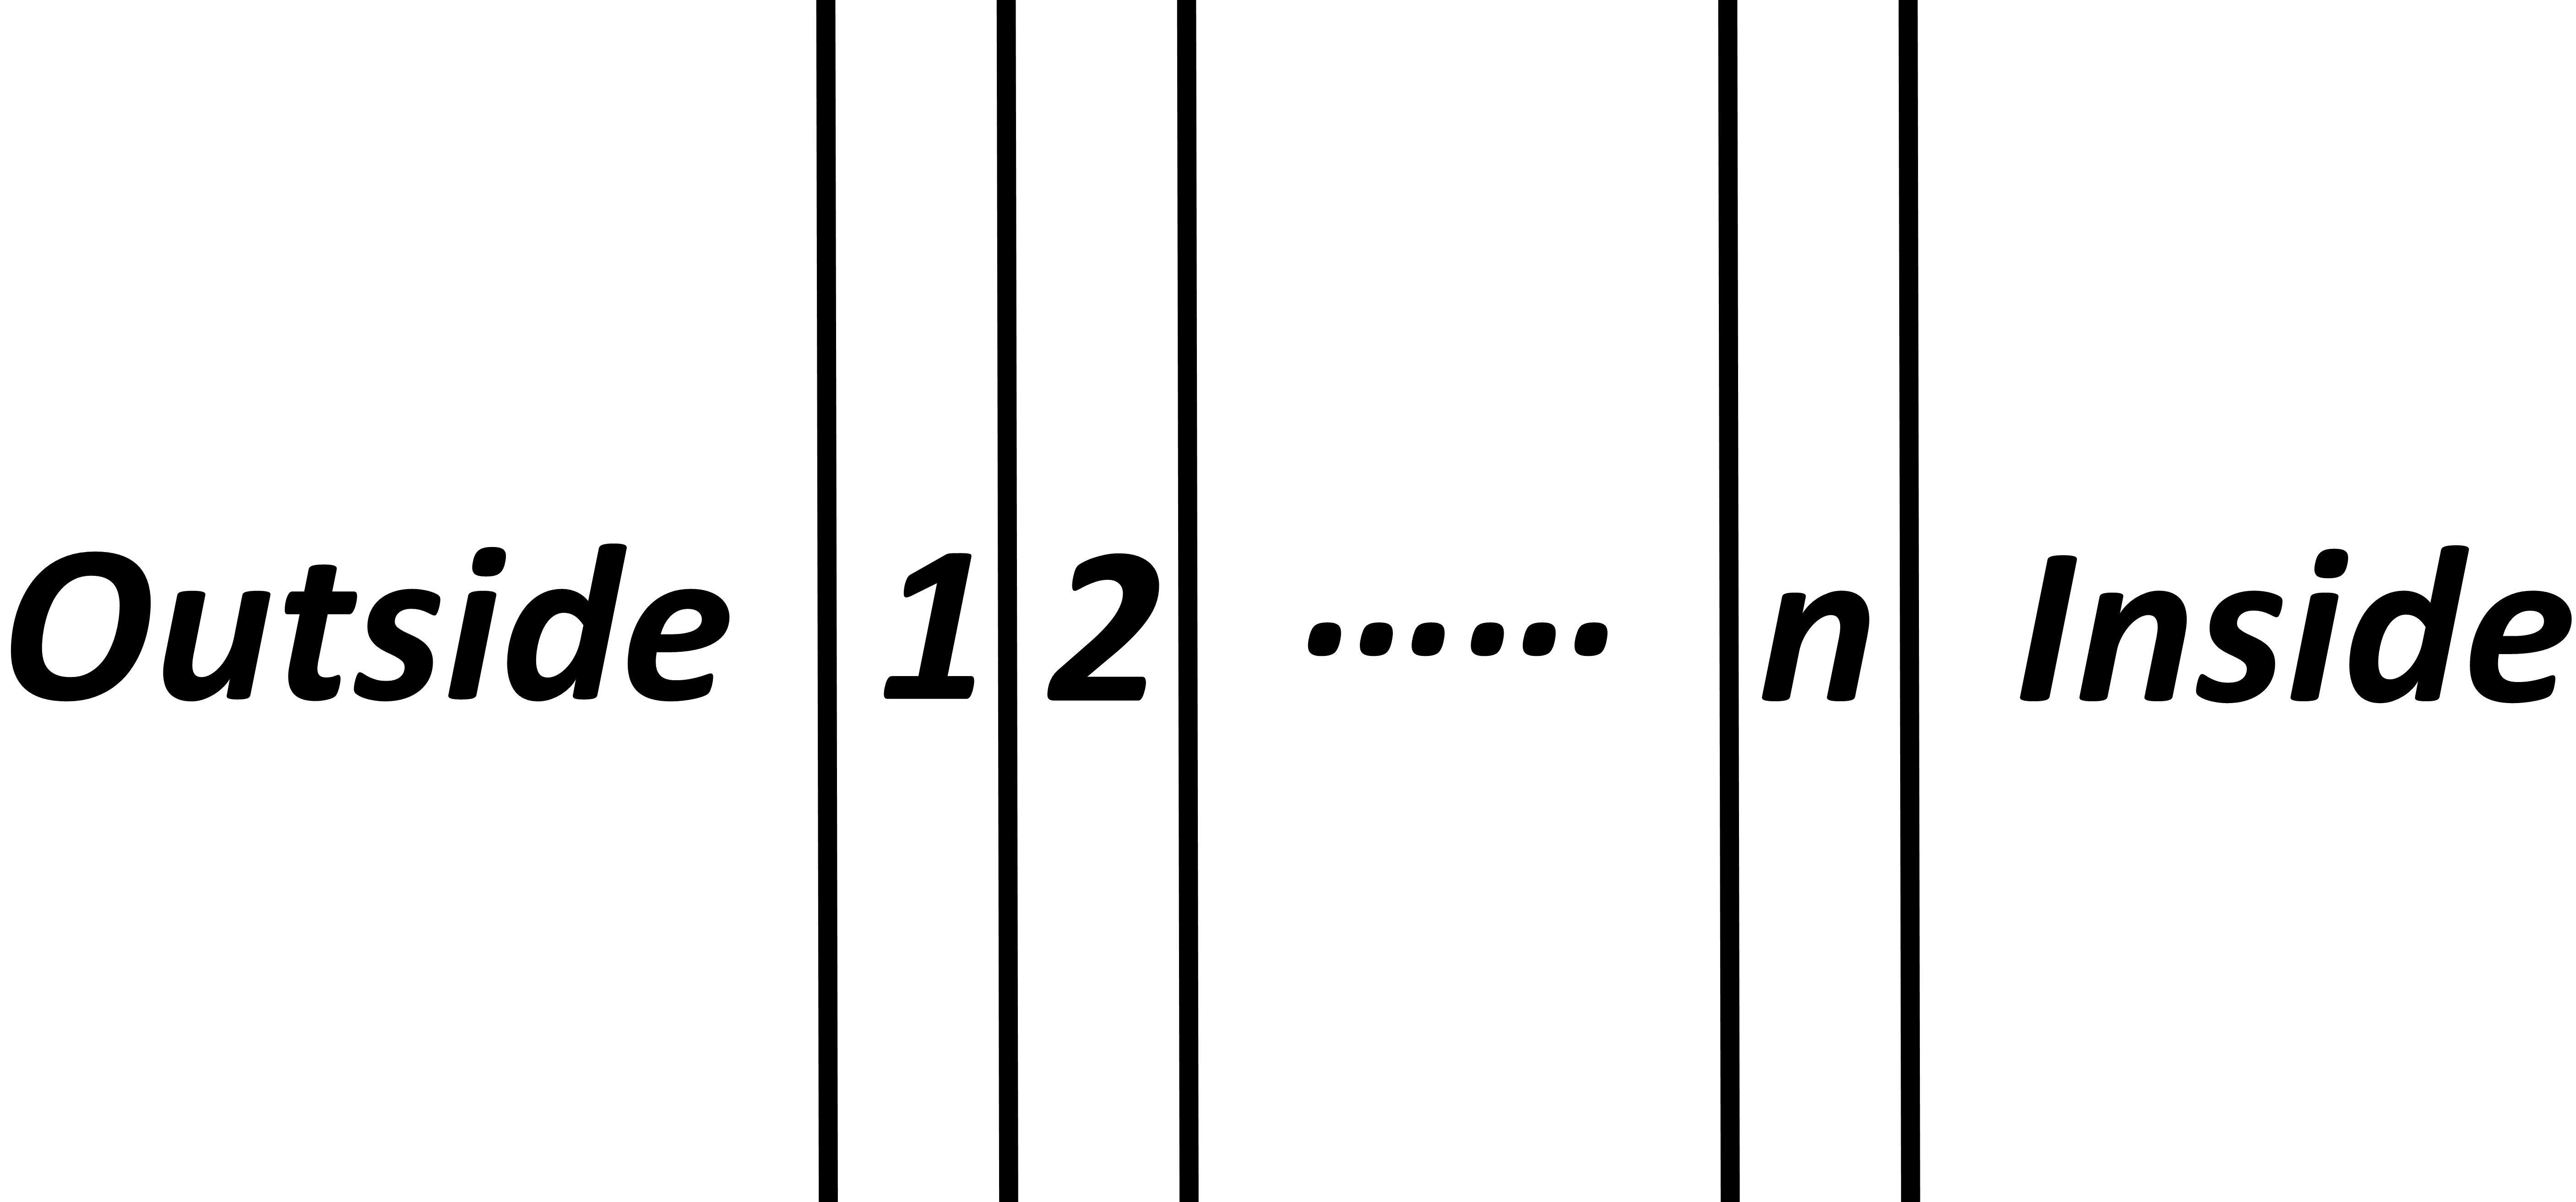
\includegraphics[width=2.3in,keepaspectratio]{./figs/background_walls.jpg}
\caption{Construction element layers}
\label{fig:background:walls}
\end{figure}

\begin{figure}[h]
\centering
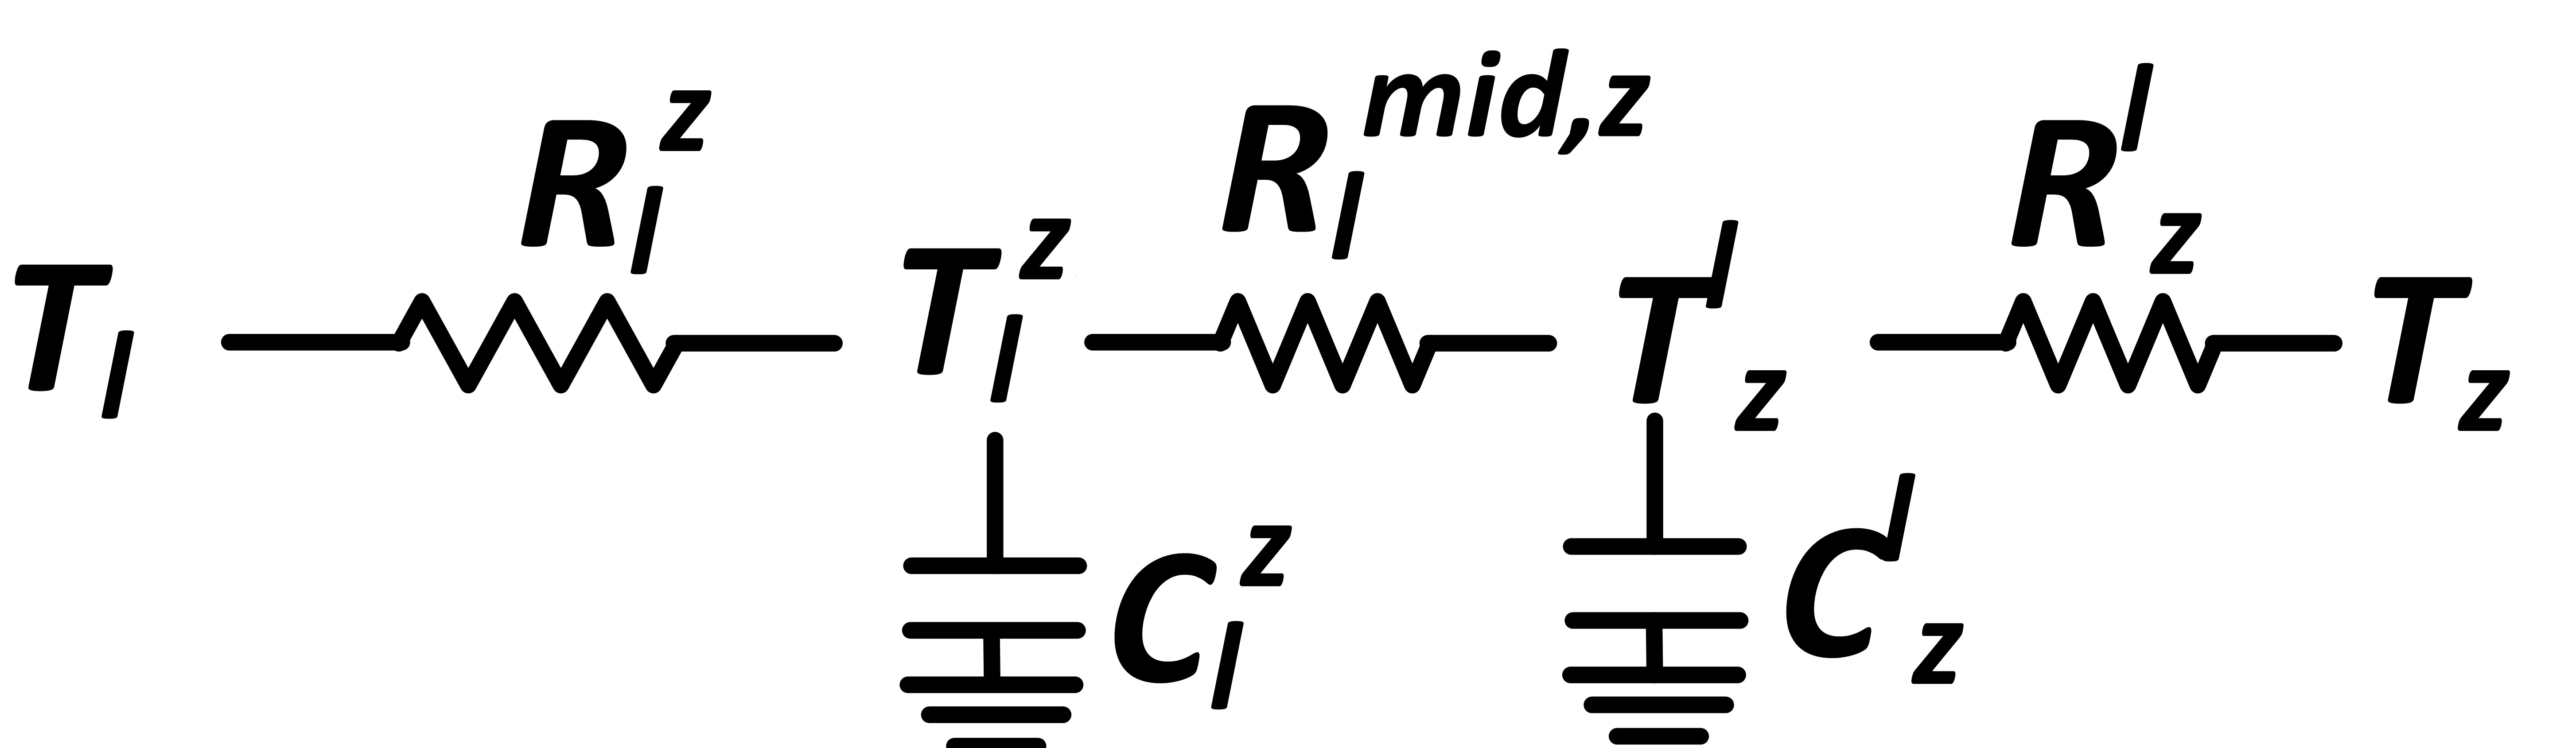
\includegraphics[width=2.3in,keepaspectratio]{./figs/background_rc.jpg}
\caption{Lumped parameter construction element}
\label{fig:background:rc}
\end{figure}

$T_l^z$ and $T_z^l$ represent the temperatures within the construction element. $T_l$ and $T_z$ represent the room temperatures at two adjacent zones. The total thermal resistance $R_{total}$ and the total thermal capacitance $C_{total}$ of each construction element can be calculated by the following equations:
\begingroup
\begin{align*}
R_{total} &= \left(\sum_{l=1}^{l=n} \frac{x_l}{k_l} \right) / A \\
C_{total} &= A \times \left( \sum_{l=1}^{l=n} x_l \times \rho_l \times c_l \right)
\end{align*}
\endgroup

\noindent where $R_{total}$ is the sum of $R^z_l$, $R^{mid,z}_l$ and $R^l_z$, and $C_{total}$ is the sum of $C^z_l$ and $C^l_z$. $A$ is the area size of a wall, $x_l$ is the length of the layer $l$ measured on a path parallel to the heat flow, $k_l$ is the thermal conductivity, $\rho_l$ is the density and $c_l$ is the specific heat capacity of the material at layer $l$.
The state equations for the thermal behaviour of each construction element can be written as follows:
\begingroup
\begin{align*}
C_l^z \dot{T}_l^z &= \frac{1}{R_l^z}\left(T_l-T_l^z\right) + \frac{1}{R_l^{mid,z}}\left(T_z^l-T_l^z\right) \\
C_z^l \dot{T}_z^l &= \frac{1}{R_l^{mid,z}}\left(T_l^z-T_z^l\right) + \frac{1}{R_z^l}\left(T_z-T_z^l\right) \\
C_l \dot{T}_l &= \frac{1}{R_l^z}\left(T_l^z-T_l\right) + Q^p_l + Q^s_l
\end{align*}
\endgroup

Note that $C_l$ denotes the thermal capacitance in room $l$, $Q^p_l$ denotes the internal heat gain from occupants and $Q^s_l$ denotes the solar heat gain.

The model order is equal to the number of capacitors used (i.e. number of \textsl{C}'s used) and for every \textsl{C}, the governing equation includes a linear differential equation. 
The resulting linear differential equation for each element can be solved analytically, making the method very computationally efficient. However, note that the model complexity increases along with the number of capacitors used. 
Thus, the capacitance and its corresponding resistances have to be carefully chosen to model the combined effect of conduction between the air masses separated by the surface, as well as radiation and convection between the surface and the air mass in contact with it \citep{goyal2012method}. 

\cite{gouda2002building} showed that a second-order lumped RC-network model with 3 resistors (\textsl{R}) and 2 capacitors (\textsl{C}) is sufficient to capture the thermal dynamic interaction between two spaces connected through a single wall. 
They showed that a reduced model based on second-order building element gives minimal loss of accuracy but significant improvements in computational effort compared to a baseline model of twenty-order lumped RC parameters benchmark. 
Thus it is possible to model the thermal interactions in a multi-zone building by using such simpler 3R2C-networks as building blocks. 

%%In this formulation, the building is represented by a network graph with nodes and edges, as in Figure \ref{fig:background:rc_network}. 
%%A node may represent a physical zone (e.g. a room, a hallway, an outdoor space) or some point inside a wall. 
%%Edges represent pathways for conductive heat flow. 
%%The air in a zone is assumed to be well-mixed so that each zone is characterised by a single temperature. 
%
%%Using these R's and C's, the network can be represented graphically as shown in Figure \ref{fig:background:zones} and Figure \ref{fig:background:rc_network}. 
%%For a zone with four adjacent walls, a window, a ceiling and a floor as depicted in Figure \ref{fig:background:zones}, the RC-network models are represented in Figure \ref{fig:background:rc_network}. 

The configurations of thermal capacitance and thermal resistances for each building elements modeled are essential. To identify the value of these parameters, three different methods can be employed:

\emph{White-box model}: This approach has a strong physical basis. The RC network's topology as well as its R and C elements (the model parameters) are derived directly from detailed geometry and construction data. For each construction element making up the building space, the layering materials, thickness, thermal conductivity, specific heat capacity and density are identified. The values of the total resistance and capacitance for each element are first calculated, and further divided into three resistance fractions and two capacitance fractions \citep{gouda2000low,gouda2002building,deng2010building,dobbs2012automatic,goyal2012method,sturzenegger2012semi,sturzenegger2014brcm}.

\emph{Black-box model}: Due to the complexity of underlying physics, a data driven approach that identifies building thermal dynamics  interactions from observed behavior is widely explored \citep{goyal2011identification,cigler2013beyond,zhou2016quantitative}. These data-driven models use techniques such as Kalman Filtering and semiparametric regression to learn the parameters of the RC network. This approach is conceptually simple but depends crucially on the availability of appropriate input data sets that encompass sufficient long sequences of all relevant feedback-response signal pairs. These are very hard to obtain from a real building during normal operation.

\emph{Grey-box model}: This first specifies a plausible RC network model using the white-box approach \citep{cigler2013beyond,ghosh2015modeling}. The model parameters are then further fitted to the building thermal dynamics using the measurements data. The advantage of this approach is that basic knowledge about possible thermal interactions can be easily introduced, and the model parameters are fitted further to a specific buildings. 


%\begin{figure}[h]
%\centering
%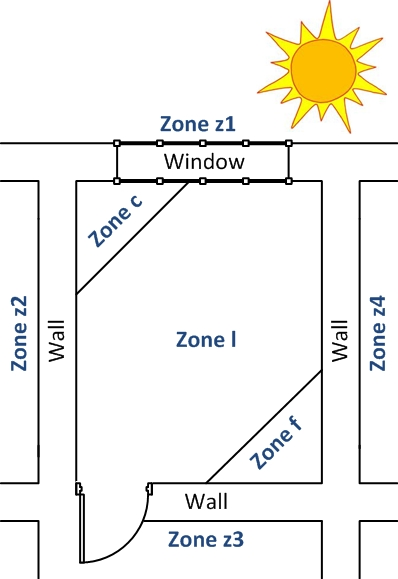
\includegraphics[width=2.3in,keepaspectratio]{./figs/zone1.jpg}
%\caption{Building with 4 zones}
%\label{fig:background:zones}
%\end{figure}
%
%\begin{figure}[h]
%\centering
%\includegraphics[height=2.3in,keepaspectratio]{./figs/background_3r2c.jpg}
%\caption{Lumped-RC network for 4 zones}
%\label{fig:background:rc_network}
%\end{figure}
%
%Figures \ref{fig:background:zones} and \ref{fig:background:rc_network} show a scenario example using lumped RC network to model the building thermal dynamics. In this formulation, a zone with four adjacent walls, a window, a ceiling and a floor ($z \in Z = {z1, z2, z3, z4, f, c}$), as depicted in Figure \ref{fig:background:zones}, is represented by a network graph with nodes and edges, as in Figure \ref{fig:background:rc_network}. A node may represent a physical zone (e.g. a room, a hallway, an outdoor space) or some point inside a wall. Edges represent pathways for conductive heat flow. The air in a zone is assumed to be well-mixed so that each zone is characterised by a single temperature.

In Chapter \ref{cha:milp} Section \ref{mip:thermal}, we adopt this lumped RC method and present a complete state-space formulation of the thermal dynamics of a building. Specifically, we use a white-box model in the settings of R's and C's. In Section \ref{cha:ep} of the Appendix, we compare our model with building energy simulation software using a grey-box model.  

The lumped RC methods have been well-explored in the recent years as they are more accurate and computationally efficient \citep{gouda2000low,gouda2002building,goyal2012method,goyal2011identification,deng2010building,ghosh2015modeling,sturzenegger2014brcm,dobbs2012automatic,ma2012demand,eisenhower2012uncertainty,radecki2012online}. Due to its practicality, this model has been widely employed by various MPC-based HVAC control mechanisms \citep{goyal2012method,goyal2011identification,ma2012demand,sturzenegger2012semi,cigler2013beyond}. We refer the readers to \citep{kramer2012simplified} for a comprehensive review of building thermal models. %the lumped RC methods as a simplified model that is near-accurate and reduces computational time is practical for MPC-based HVAC control. 

\subsection{Building Energy Software Simulation}

It is worth noting that in the HVAC community, building energy simulation software such as EnergyPlus \citep{crawley2000energyplus}, TRNSYS \citep{university2010trnsys} and DOE-2\/eQuest \citep{hirsch2010equest} are typically used for modeling building thermal behaviors. These tools contain numerous complex calculations that are useful for load calculations, equipment sizing, and predicting energy use of a building over long time intervals. However, their utility is limited as tools to model or simulate the dynamics of the thermal processes inside a building that can be used by a control system \citep{goyal2011identification}. Due to the software complexity, it is hard to seamlessly integrate optimisation algorithms with these simulation software.

Several works have also been done to compare the lumped RC model with EnergyPlus \citep{sturzenegger2012semi,dobbs2012automatic,eisenhower2012uncertainty}. \citep{sturzenegger2012semi} concludes that the understanding of wall materials and their built-up is essential to build an accurate RC model. Nonetheless, \citep{eisenhower2012uncertainty} further states that the reduced lumped RC network is robust to the uncertainty in the RC parameters of the model, and \citep{dobbs2012automatic} demonstrates that the use of model aggregation reduces computational time without significant loss of accuracy.

% Refer \citep{dobbs2012automatic} to improve on writing RC

\section{Occupancy Modeling} \label{cha:bg:occ} 

%Building occupancy varies dynamically. 
Building occupancy changes over time. 
Conference rooms, cafeterias, auditoriums, and other assembly spaces are often unoccupied for significant periods of time. Office occupancy varies during the course of a work day, from day to day, and over longer terms because of attendance of meetings elsewhere, business travel, changing room functions, and variations in staffing. The resulting over-ventilation,
during times when the space has less than maximum occupancy or is unoccupied, wastes significant HVAC energy and causes discomfort for occupants in some spaces (e.g., conference rooms) from over-cooling or overheating. In a dynamic environment where the zone settings and occupancy keeps changing, knowing occupancy information, including whether a zone is occupied or vacant, the number and identities of the occupants, is essential for occupancy-based HVAC control \citep{erickson2010occupancy,nguyen2013energy}. Thus, various mechanisms have been developed to detect, monitor, model and predict occupancy in each zone. 

\subsection{Fixed Schedule}

The most basic technique for indicating occupancy in the building involves a programmable schedule that is customizable and takes into account the occupant's activity/business hours, special events such as business trips, leaves and holidays. The HVAC system is turned on and off based on these fixed system schedules. 

\subsection{Sensor-based Occupancy Detection}

An improvement of this technique uses motion detection or Passive infrared (PIR) sensors \citep{agarwal2010occupancy} to verify whether or not occupants really are in office spaces during the scheduled times. If no motion is detected within a set time, action is taken such as changing the setpoints, or reducing minimum air flow rates into the zone \citep{zhang2013energy}. %The setback of using motion sensors is that these sensors are limited to movement and does not detect actual occupancy in a given area. 
Motion detectors provide an efficient way to detect occupancy, but they provide no information about the number of people using the space. This finer-grained information is essential to perform demand-driven temperature control and $CO_2$ ventilation. More comprehensive sensors-based and vision-based systems have been developed to achieve this goal. These systems use temperature sensors, humidity sensors, $CO_{2}$ sensors, acoustic sensors, ambient light \citep{chang2013statistical}, wireless cameras \citep{erickson2009energy}, door state sensing \citep{agarwal2010occupancy,hutchins2007modeling}, RFID \citep{li2012measuring}, communication network infrastructures \citep{melfi2011measuring,zeiler2012wireless} or combinations of various sensors \citep{yun2012building,mamidi2012adaptive,lam2009occupancy,dong2009sensor,meyn2009sensor,barakat2016agent,pedersen2017method} to provide better measures of actual occupancy. Detailed surveys of these occupancy detection systems can be found in \citep{labeodan2015occupancy,liu2012review}.

% However these sensing systems have strong dependencies on body heat accumulation and $CO_2$ concentration, which take time to build up and are a cumulative effect of various factors other than occupancy such as outdoor air quality and ventilation rate. While these systems are suitable for understanding general trends at longer time scales, they fail to respond quickly to ever changing occupancy.

%More advanced systems have been deployed, such as using cameras and vision algorithms. Extensive research has been conducted on developing occupancy detection system tat is accurate, inexpensive and easily deployable within existing buildings. 

\subsection{Occupancy Prediction}

While real time occupancy monitoring is important, occupancy prediction is also helpful for HVAC control especially with MPC. Time is required for rooms to be brought to appropriate temperatures, therefore the conditioning of the room must begin prior to when the room is actually utilised. This cannot be achieved solely by depending on real time occupancy detection. The capability of predicting occupant movement or room usage patterns is crucial to trigger HVAC control at a timely manner. %based on the estimated occupancy of a zone. 
For example if a lobby has a large number of people, then the HVAC system might predict that an adjacent conference room will be used with high probability and begin conditioning before people actually enter the room.

Various methods have been developed to understand the dynamics of occupancy patterns. The spatiotemporal dynamics of occupancy has high variability that makes this a challenging task. Determining the number of people that occupy a particular space and the corresponding duration are difficult to characterise because human behavior is considered stochastic in nature. For example, occupants do not arrive and leave at the same time of the day, their locations within the building also vary throughout the day. As a result, different zones have different hourly occupancy rates on different days. To model these occupancy behaviors and movement patterns in buildings, different approaches have been investigated and explored. These include 
\begin{itemize}
	\item statistical techniques \citep{clevenger2006impact,page2008generalised,erickson2009energy,nassar2010model,goldstein2011space,liao2011novel,duarte2013revealing,chang2013statistical}, 
	\item machine learning techniques \citep{lam2009occupancy,yu2010modeling,yang2016building} and
	\item graphical model approaches \citep{hutchins2007modeling,dong2009sensor,meyn2009sensor,erickson2010occupancy,liao2010integrated,kamthe2011enabling}.
\end{itemize}
These mechanisms learn behavioral patterns from occupancy data collected from sensors and vision cameras. Based on the occupancy data, different occupant diversity profiles describing the occupancy distribution of each zone are created. Specifically, the occupancy profiles reflect the time-series information for each zone, for example 
\begin{enumerate*}[label=(\roman*)]
	\item first arrival and last departure times of the occupants,
	\item estimated number of occupants per hour for each day, %cumulative presence per hour for each work day
	\item periods of intermediate presence and absence, and	
	\item occupant mobility patterns in buildings.
\end{enumerate*}

These occupancy profiles contain valuable information when deciding demand control strategies: they enable occupancy-based control to forecast the density of people at each zone. Predicted occupancy (number of people) can be converted to the zone thermal loads, thereby enabling the HVAC system to operate dynamically, such as using different temperature setpoints and ventilation rates on a zone by zone basis at each day and time. %Specifically, how such occupancy information are utilised in the HVAC system varies amongst different HVAC control systems. 

\subsection{Meeting/Timetable Scheduling}

\begin{table*}[t]
\centering
\begin{tabular}{p{0.3\linewidth} p{0.1\linewidth} p{0.08\linewidth}  p{0.08\linewidth} p{0.08\linewidth} p{0.08\linewidth} p{0.08\linewidth}}
\hline\centering{ } & \centering{\cite{majumdar2012energy}} & \centering{\cite{kwak2013tesla}} & \centering{\cite{pan2012thermal}} & \centering{\cite{klein2012coordinating}}  & \centering{\cite{chai2014minimizing}} & \centering{\cite{balaji2013zonepac}}\tabularnewline
\hline  \emph{Ad-hoc/Fixed Schedule} &  &  &  &  &  &  \tabularnewline
\hline  Brute force & \centering{x} &  &  &  &  &  \tabularnewline
\hline  Random room & \centering{x} &  &  & \centering{x} & \centering{x} & \centering{x} \tabularnewline
%\hline  Maximum room & \centering{x} &  &  &  &  &  \tabularnewline
%\hline  Minimum room & \centering{x} &  &  &  &  & \tabularnewline
%\hline   &  &  &  &  &  &  \tabularnewline
%\hline  \emph{Greedy Approach} &  &  &  &  &  &  \tabularnewline
%\hline  Time gap & \centering{x} &  & \centering{x} &  &  &  \tabularnewline
%\hline  Capacity gap & \centering{x} &  & \centering{x} &  &  &  \tabularnewline
%\hline  Time gap + capacity gap & \centering{x} &  &  &  &  &  \tabularnewline
\hline   &  &  &  &  &  &  \tabularnewline
\hline  \emph{Optimisation Approach} &  &  &  &  &  &  \tabularnewline
\hline  Search Techniques &  &  &  &  &  &  \tabularnewline
\hline  \hspace{5pt} Greedy &  &  & \centering{x} &  &  &  \tabularnewline
\hline  \hspace{5pt} Hybrid greedy & \centering{x} &  &  &  &  &  \tabularnewline
\hline  A* search & \centering{x} &  &  &  &  &  \tabularnewline
\hline  Mixed integer programming &  & \centering{x} &  &  & \centering{x} &  \tabularnewline
\hline  Markov decision problems &  &  &  & \centering{x} &  &  \tabularnewline
\hline   &  &  &  &  &  &  \tabularnewline
\hline  \emph{Heuristics} &  &  &  &  &  &  \tabularnewline
\hline  Room occupied duration & \centering{x} &  &  &  &  &  \tabularnewline
\hline  Number of room used & \centering{x} &  &  & \centering{x} &  &  \tabularnewline
\hline  Time gap & \centering{x} &  & \centering{x} &  & \centering{x} &  \tabularnewline
\hline  Capacity gap & \centering{x} & \centering{x} & \centering{x} &  & \centering{x} &  \tabularnewline
\hline  Key meeting &  & \centering{x} &  &  &  &  \tabularnewline
\hline  Non-peak time &  & \centering{x} &  &  & &  \tabularnewline
\hline  Real-time pricing &  &  & \centering{x} &  & \centering{x} &  \tabularnewline
\hline   &  &  &  &  &  &  \tabularnewline
\end{tabular}
	\caption{Existing energy-aware meeting/timetable scheduling approaches}
	\label{tab:sche_appr}
\end{table*}

While building occupancy flows are naturally stochastic, some studies try to schedule activities such as meetings and lectures in order to deterministically control occupancy flow in an energy optimum fashion. Such energy aware occupancy scheduling approaches have gotten more attention in recent years due to the significant cost saving opportunities. Even simple rules like consolidating meetings in fewer buildings have proven to be very effective. For example, Portland State University consolidated night and weekend classes that were held across 21 buildings into 5 energy efficient buildings. By doing so, they reported a reduction of 18.5\% in electricity consumption over the fall season compared to the previous three-year average \citep{portland:2012}. Significant savings have also been reported by several other universities \citep{msu:2009,ncu:2015,iowa:2015} which deployed the same strategy during their summer school term by compacting schedules and consolidating the use of classroom space strategically.

\cite{balaji2013zonepac} and \cite{capehart2007web} optimise HVAC control based on user input schedule from meeting appointment systems such as Microsoft Outlook. This approach assumes exact meeting schedules and therefore it is equivalent to the fixed schedule approach. The drawback of this approach is that it basically ignores that some schedules might lead to more energy savings.

Another work focuses on optimising meeting scheduling and timetabling based on a heuristic approach. Table \ref{tab:sche_appr} presents a summary of the existing work on energy-aware occupancy scheduling. These works look into the aspect of occupancy scheduling, and focus on generating energy-efficient schedule based on heuristics. They examine various configurations of meeting schedules using different approaches to identify the best schedule that minimise energy used while observing the meeting constraints.

\cite{majumdar2012energy} evaluate the performance of a number of scheduling algorithms that they run through the building energy simulation software EnergyPlus \citep{crawley2000energyplus}. They first adopt a brute force method to explore all possible room choices for a small set of meetings using depth-first search. To identify an energy-efficient schedule, they then calculate the energy consumption of each solution found using EnergyPlus. This makes the brute-force method computationally impractical. To generate a practical baseline benchmark, they resort to a random room assignment approach. Their algorithm performs depth first search to randomly assign each meeting to a room, until all the meetings are scheduled. At any stage, it backtracks to the previous solution in case no feasible room option is available. Amongst all of the existing work, random room assignment appears to be a commonly adopted approach to generate benchmark performance, which we also observe in the work by \cite{klein2012coordinating} and \cite{chai2014minimizing}.

To generate an energy-efficient schedule, \cite{majumdar2012energy} introduce a set of heuristics in their energy cost model. 
%They use various factors to approximate the energy-optimality of a meeting schedule, such as room occupied duration, number of room used, time gap between successive meetings in the same room, capacity gap between the room size and the meeting size. 
Such heuristics include room occupied duration, number of rooms used, time gap between successive meetings in the same room, capacity gap between the room size and the meeting size are used to approximate the energy-optimality of a meeting schedule. 
Guided by this set of heuristics, they use hybrid greedy search to greedily commit to the minimum cost schedule. They also adopt such heuristics to guide A* search by pruning suboptimal search trees. The former performed best when considering only one criterion, but a more involved A* search with successive calls to EnergyPlus performed best overall.

\cite{pan2012thermal} consider a similar approach. Some criteria considered in their algorithms include minimising the number of rooms, minimising time between meetings in the same room, and minimising room size. By adopting a greedy-based approach guided by such heuristics, they show that by scheduling meetings back-to-back in the same room, a 20\% energy savings is observed when comparing results to existing schedules. They also consider another approach of minimising energy cost based on real-time pricing in \cite{pan2013minimizing}.

The work by \cite{kwak2014building} and \cite{chai2014minimizing} are the closest to our work. Unlike \cite{majumdar2012energy} and \cite{pan2012thermal}, they adopt a mixed integer programming approach to schedule meetings in an optimal manner. However, they consider similar heuristics criteria such as minimising time gap between successive meetings in the same room, minimising capacity gap between the room size and the meeting size. It is important to note that these works minimise energy use without directly modeling the HVAC system. In our work we integrate occupancy scheduling with HVAC control, because it is of key importance to determine which rooms need to be heated or cooled and when. For example, sometimes it is more energy efficient to pre-cool a room rather than cool it at the time of a meeting. In order to determine the HVAC operation one needs to decide the HVAC control settings.

\cite{klein2012coordinating} look at a slightly different perspective on energy-aware scheduling. They develop a multi-objective Markov Decision problems to coordinate both HVAC system and building occupants through meeting relocations. In order to generate an energy-efficient schedule, their multi-agent system attempts to re-locate meetings into minimum number of rooms within similar zones through meeting agents. Similarly, \cite{kwak2014building} also develop an agent-based system to interact with the occupants to reschedule meetings and incentivise them based on their energy saving activities. While the human behavior aspect is out of the scope of this thesis, these existing works address an important problem and its solution that can be integrated with our work to form a complete solution.

In Chapter \ref{cha:milp} we combine meeting/timetabling scheduling with occupancy-based HVAC control, and show how the joint model can outperform these state-of-the-art approaches.

%subclassify : heuristics (minimising...), tree search algorithm (use heuristics to prune tree, read majumdar) + EP at the leaf of search to compare schedule, MIP + black box model (eg. energy data, not EP), 

%Cons: many meetings occur spontaneously with no pre-scheduling in Outlook 

%to formulate an en However, they use MIP to calculate an energy efficient schedule assuming black-box modeling of the HVAC control.   Similar criteria are considered in the work by

%HVAC control design and operation such as ventilation control based ont he results of detected number of occupants.
%calculate a zone thermal loads and thus correctly size and provision HVAC system.
%predict room usage thereby enabling us to control the HVAC systems in an adaptive manner
%predict occupancy (number of people) in a building (or zone) as a function of time given some initial condition. Such predictions can serve as inputs to HVAC control.

%Diversity factor are hourly fraction for a 24-h day \citep{duarte2013revealing}. A profile for each of the week can be created and combined to make up a representative week of general occupancy or specific equipment operation profiles in a building. The diversity factor for each workweek, generally Monday though Friday, are often treated identically with weekend days having a different profile. Alternatively, each day of the week can be differentiated in order to represent intricacies in occupancy or equipment operation profiles in an office building. In the same way each zone type will often have different profiles in order to represent the intended use of the space with regards to energy factors. The profiles have a range from zero to one where zero represents no usage of the equipment or no people in the zone and one represents peak equipment usage or the maximum design level of people in the building or zone. In the case of HVAC equipment, the occupancy diversity factor is used to multiply the design cooling/heating load in an energy simulation because occupancy will not always be at the maximum design level and it is a way to account for the variable heat gains throughout the day. Diversity factors are lower during hours when people are not present and ramp to a maximum value during hours when people are most present or when weather is at or beyond an extreme design condition.

%Due to the random nature of individual's behavior and challenges accessing accurate data, current studies include the creation of deterministic schedules where a standard workday profile is the same or the whole workweek and both weekend days have the same profile. Depending on the available data,, this method assumes no change in occupancy schedules throughout the year. These are referred as deterministic models. In more complex and sophisticated stochastic occupancy models, schedules for one week are not the same as the next. Stochastic models use various probabilistic methods to create the dynamic schedules. 

% Temperature control has a long response time to power state changes and demands a predictive approach.
% Sensor measurements alone are not enough for accurate estimation since they suffer from large measurement error.
% Fusing sensor data with model prediction is essential.
% Due to the highly uncertain nature of occupancy dynamics, modeling and estimation of occupancy is a challenging problem.
% Filtering techniques can be used to compensate for measurement error by fusing noisy sensor measurement with prediction from a model. This requires a model of occupancy dynamics. 
% a model of occupancy dynamics 
%Several stochastic models have been developed to model occupant presence and interactions with space appliances and equipments such as lighting, random opening of windows,



\section{Thermal Comfort} \label{cha:bg:atc} 

Thermal comfort is the condition of mind that expresses satisfaction with the thermal environment and is assessed by subjective evaluation \citep{ashrae2013thermal}. Individuals vary greatly in their physiological reaction to their thermal environment. Perception of thermal comfort is affected by many factors, including air temperature, air speed, humidity, clothing, the amount of physical exertion and outdoor temperature \citep{bradshaw2010human}. Under the same thermal conditions, some individuals may feel too hot, while others wearing identical clothing feel too cold. Because there are large variations, both physiologically and psychologically, from person to person, it is difficult to satisfy everyone in a space. Consequently, standards are defined to specify the combinations of indoor thermal environmental factors and personal factors that will produce thermal conditions acceptable to a majority of the occupants within the space. 

\subsection{Fixed Comfort Setpoints}

\cite{ashrae2013thermal} defines a standard for thermal environmental conditions suitable for human occupancy. It addresses the interactions between temperature, thermal radiation, humidity, air speed, personal activity level, and clothing. The standard recommends conditions that have been found experimentally to be acceptable to at least 80 percent of the occupants within a space. The operative temperature range for building occupants in typical winter clothing %(0.8 to 1.2 clo)
 is specified as 20$^\circ$C to 23.5$^\circ$C. The preferred temperature range for occupants dressed in summer clothes %(0.35 to 0.6 clo)
 is 22.5$^\circ$C to 26$^\circ$C. These values are derived from the Predicted Mean Vote (PMV) method developed by \cite{fanger1970thermal}. PMV is an index that predicts the mean value of the thermal sensation votes (self-reported perceptions) of a large group of persons on a sensation scale expressed from -3 to +3 corresponding to the categories cold, cool, slightly cool, neutral, slightly warm, warm and hot.
This method treats all occupants the same and disregards location and adaptation to the thermal environment. It basically states that the indoor temperature should be a fixed configuration. This is taking the more passive stand that occupants do not have to adapt to different temperatures (since the temperature will always be constant). As a consequence, the PMV-based static thermal model incurs high HVAC operating cost as substantial energy is being consumed to ensure fixed thermal comfort range.

\subsection{Adaptive Comfort Setpoints}

As energy savings are becoming a priority in building operations, a number of studies started to investigate the potential of energy reductions that can be delivered by the use of adaptive comfort setpoints \citep{mui2003adaptive,egan2010the,schumann2010learning,ward2010automate,yang2013development,west2014trial,chew2015adaptive}. It is first shown in \cite{de1998developing} that occupant response to room temperature depends on outdoor temperature. According to them, people in warm climate zones prefer warmer indoor temperatures than people living in cold climates zones. Similarly, in hot summer the occupants can tolerate a lot more ambient heat than in winter, because human bodies become used to the higher range of temperatures. They suggest an adaptive comfort model that correlates the outdoor temperature with indoor comfort temperature. 

\begin{figure}[b]
\centering
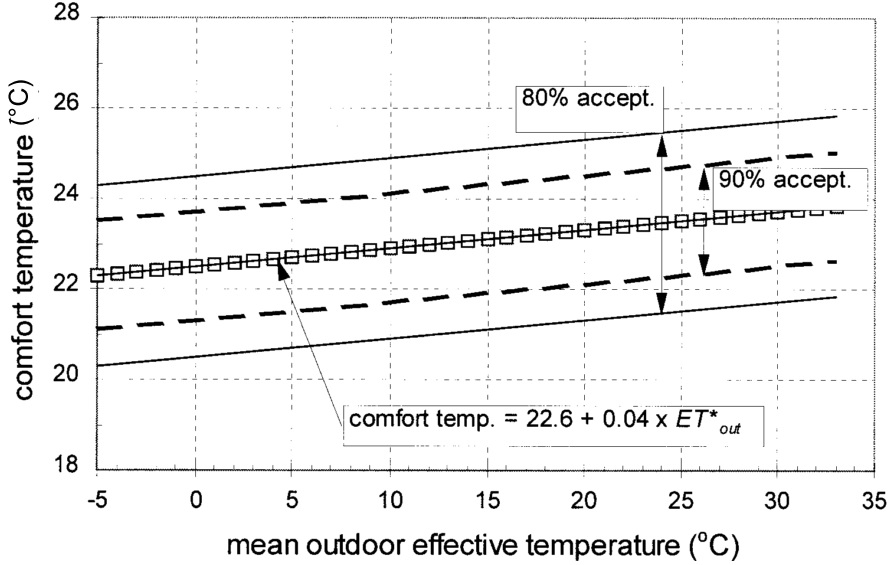
\includegraphics[width=3.2in,keepaspectratio]{./figs/dear_adaptive_thermal_model.jpg}
\caption{Adaptive comfort model for buildings with centralized HVAC and non-opening windows adapted from \cite{de1998developing}}
\label{fig:background:dear_adaptive_temp}
\end{figure}

The adaptive comfort model defines a variable temperature setpoint based on the effective temperature (ET), which is calculated based on the arithmetic average of outdoor temperature at 6 a.m. (assumed minimum daily temperature) and outdoor temperature at 3 p.m. (assumed maximum daily temperature) for a calendar month or particular days. Contrary to the static assumptions underlying the PMV method in \cite{fanger1970thermal}, their results show that occupants thermal comfort sensations are impacted by outdoor temperature, as shown in Figure \ref{fig:background:dear_adaptive_temp}. Based on this finding, numerous studies have been conducted and showed that the adaptive model leads to substantial energy reductions \citep{mui2003adaptive,egan2010the,ward2010automate,yang2013development,west2014trial,chew2015adaptive}. Adopting the adaptive model is a matter of actively managing occupant expectations influencing comfort perception and promoting thermal acceptability \citep{ward2010automate}. In Chapter \ref{cha:atc}, we present a model that allows the occupant to indicate their thermal comfort flexibility. Based on this input, we demonstrate substantial energy savings by dynamically adjusting the comfort setpoints, while providing probabilistic guarantees of thermal comfort satisfaction, considering the uncertainty in the thermal flexibility of occupants.


 
%Each countries define different standards that provide minimum requirements for acceptable indoor thermal environments \citep{vic2008workplace}.
%These standards establish the ranges of indoor environmental conditions that are acceptable to achieve thermal comfort for occupants. 
%In the US, 
%Alternately, in Australia, the optimum comfort temperature for sedentary work is defined between 20$^\circ$C and 26$^\circ$C, depending on the time of the year and clothing worn \citep{vic2008workplace}. 
%While different countries have different standards, each geographical location may account for a spread of a few degrees from the standard indoor temperatures defined above. 
%In commercial buildings, the indoor climate to be maintained is a compromise between those necessary to ensure the comfort of occupants and those necessary to avoid high operating cost due to the energy consumption. A comfort room temperature is essential to assure occupants' productivity. Studies show that productivity drops by 20\% when the employees feel either too hot or too cold in the office environment \citep{}. 


